\section{Formal Structure of the Recursive Action}
\label{sec:recursive-action-formal}

\subsection{Recursive Action Definition}

The total action across cosmological cycles is defined as a discrete sum:
\begin{equation}
\mathcal{A}_{\text{total}} = \sum_n \mathcal{A}_n,
\end{equation}
where each cycle’s action \( \mathcal{A}_n \) is defined over the recursive configuration space
\[
\phi_n \in \mathcal{C}_n = (a_n, \varphi_n, \lambda_n, E_n),
\]
with:
\begin{itemize}
  \item \( a_n \): scale factor (quantized geometry),
  \item \( \varphi_n \): scalar field configuration,
  \item \( \lambda_n = |\langle \Psi_{n-1} | \Psi_n \rangle|^2 \): memory fidelity,
  \item \( E_n = \sqrt{-\mathrm{Tr}(\rho_{\text{red}} \log \rho_{\text{red}})} \): entanglement eigenvalue.
\end{itemize}

The cycle-level action decomposes into:
\[
\mathcal{A}_n = \int d^4x \left[
\mathcal{L}_{\text{LQC}}(a_n, \varphi_n) +
\mathcal{L}_{\text{mem}}(\lambda_n) +
\mathcal{L}_{\text{ERB}}(E_n) +
\mathcal{L}_{\text{obs}}(\phi_n)
\right],
\]
where each term corresponds to gravitational dynamics, memory penalty, ER bridge interaction, and observer projection, respectively.

\subsection{Lagrangian Components}

\paragraph{(1) LQC Gravitational Sector:}
\[
\mathcal{L}_{\text{LQC}} = \frac{1}{2} G^{IJ}(q) \dot{q}_I \dot{q}_J - V(q), \quad q = (a, \varphi),
\]
with \( G^{IJ} \) the field-space metric from LQC minisuperspace.

\paragraph{(2) Memory Penalty Term:}
\[
\mathcal{L}_{\text{mem}} = -\beta^{-1} \log \lambda_n,
\]
penalizing low coherence; \( \beta \) is the inverse memory temperature.

\paragraph{(3) Bridge Entropy Term:}
\[
\mathcal{L}_{\text{ERB}} = \frac{A(\phi_n, \phi_{n-1})}{4G} + i \lambda_E I(\phi_n, \phi_{n-1}),
\]
with
\[
I(\phi_n, \phi_{n-1}) := \mathrm{Tr}[\rho_n (\log \rho_n - \log \rho_{n-1})],
\]
quantifying quantum relative entropy across cycles.

\paragraph{(4) Observer Projection Term:}
\[
\mathcal{L}_{\text{obs}} = \langle \Psi_n | \hat{O}_n | \Psi_n \rangle,
\]
representing the decoherence-weighted observer channel (Appendix~C.6.3).

\subsection{Symmetries and Variational Constraints}

The recursive system obeys the following variational principle:
\[
\delta \mathcal{A}_n + \lambda_C \delta \left( S[\rho_n] - \lambda_S \log \lambda_n \right) = 0,
\]
enforcing entropy–coherence equilibrium per cycle. Additionally:
\begin{itemize}
  \item **Bounce Symmetry:** \( \Psi_n(\phi) \leftrightarrow \Psi_{-n}(\phi) \) under time reversal,
  \item **Minimal Geometry Condition:** \( A(\phi_n, \phi_{n-1}) \geq \ell_{\text{Pl}}^2 \).
\end{itemize}

\subsection{Euler–Lagrange Equations}

Functional variation yields:

\paragraph{(1) Scale Factor Evolution:}
\[
\ddot{a}_n + \frac{\partial V}{\partial a_n} + \frac{\partial \mathcal{L}_{\text{ERB}}}{\partial a_n} = 0.
\]

\paragraph{(2) Scalar Field Dynamics:}
\[
\ddot{\varphi}_n + \frac{\partial V}{\partial \varphi_n} + \frac{\partial \mathcal{L}_{\text{ERB}}}{\partial \varphi_n} = 0.
\]

\paragraph{(3) Entanglement Field Dynamics:}
Assuming \( S(\rho_n \| \rho_{n-1}) \sim (E_n - E_{n-1})^2 \), define:
\[
V_E(E_n) := -S(\rho_n \| \rho_{n-1}) \quad \Rightarrow \quad \ddot{E}_n + \lambda_E^{-1} \frac{\partial V_E}{\partial E_n} = 0.
\]

\paragraph{(4) Memory Fidelity Constraint:}
\[
\frac{\delta S[\rho_n]}{\delta \lambda_n} = \frac{\lambda_S}{\lambda_n},
\]
indicating logarithmic penalty structure.

\paragraph{(5) Observer Constraint:}
\[
\hat{O}_n \text{ held fixed unless observer dynamics are explicitly modeled}.
\]

These equations define recursive attractor stability under entropy-filtered geometric and informational dynamics.

\subsection{Interpretation}

The recursive action unifies loop gravitational dynamics with coherence-driven memory selection. Evolution proceeds via constrained minimization:
\begin{itemize}
  \item Coherent paths are favored by entropy-penalized interference,
  \item Decohered branches are suppressed via memory-cost divergence,
  \item Entanglement modulates bridge transfer amplitude and radiation balancing,
  \item Observer effects encode structural projection without external agents.
\end{itemize}

\textbf{Conclusion:} Recursive evolution is governed not by unconstrained dynamics, but by a memory-preserving action. The universe retains only those configurations that minimize informational tension while maintaining structural coherence.

\begin{figure}[H]
\centering
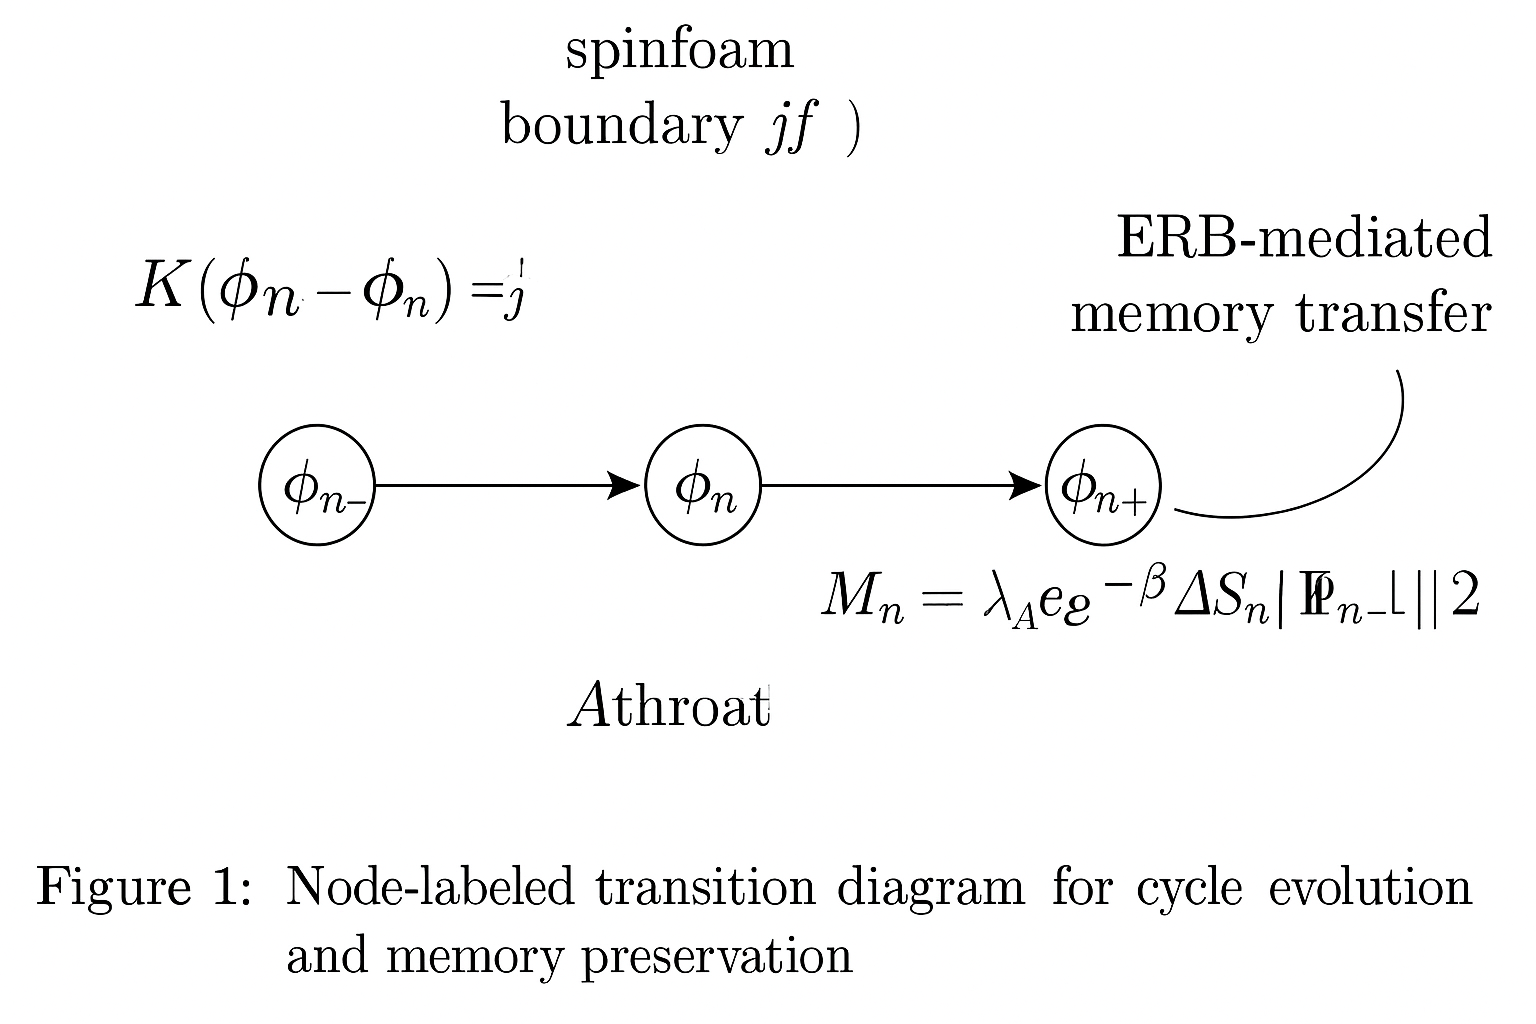
\includegraphics[width=0.75\textwidth]{figures/recursive_action_layers.png}
\caption{Layered structure of the recursive action. Each cycle contributes LQC dynamics, memory penalties, ER bridge entropy terms, and observer constraints. Recursive stability is enforced via coherence filtering and entropy balance.}
\label{fig:recursive-action-layers}
\end{figure}
